\subsection{Static verification}
	With all the geometrical values known, it has been possible to carry out a more detailed analysis. Considering a more complex model of the forces that takes into account also the distributed load due to the gravity and that the force $F$ is applied with an eccentricity $e=5cm$, it has been possible to parametrically define the hyperstatic variables as
	\[ X_1 \simeq \big( 0.63-0.16\zeta\big) N\cdot m \qquad X_2 \simeq -8.10 \ N\cdot m \] \[ X_3 \simeq \big( - 10.54 - 11.07\zeta + 55.53\zeta^2 - 6.17\zeta^3 \big) N\cdot m \]
	Evaluating the stress state on the 3 beams making up the structure for values of $\zeta \in [0,L]$, what we obtained is that the most critical section is in the elevated track for $\zeta^* = 1.65m$ at $z^* = 1.65m$ where the maximum bending value $M_x^* \simeq 135.64N\cdot m$ is achieved (as showed in figure \ref{fig:bending}). Knowing that $N^* = 0$ and neglecting the shear stress contribution due to both shear $V_y^* \simeq 111N$ and torque $M_z^* \simeq 1.89N\cdot m$, the stress state is
	\[ \sigma_{zz}(y) = \frac{M_x^*}{I_{xx,track}}y \qquad \Rightarrow \qquad \sigma_{zz,max} = \sigma_{zz}(2cm) \simeq 28.68 MPa   \]
	\begin{figure}[b]
		\centering 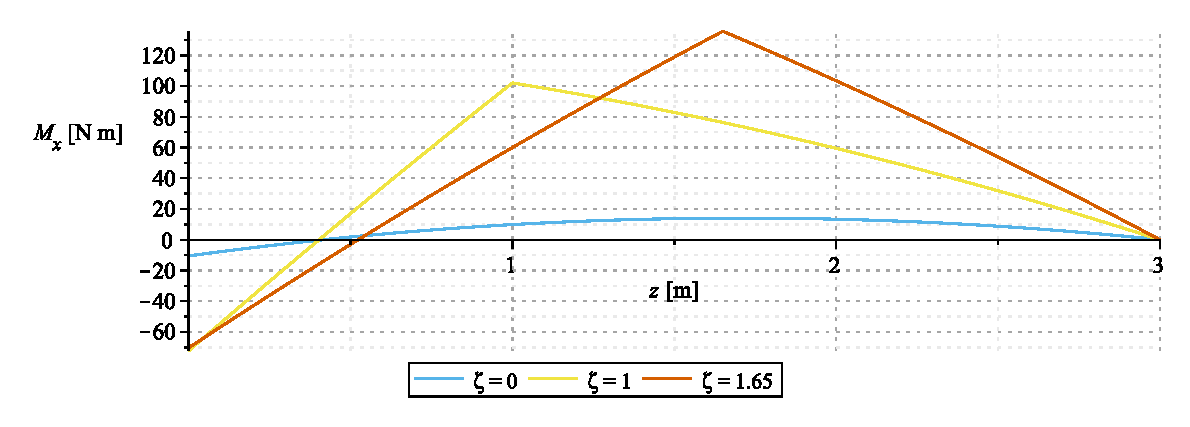
\includegraphics[width=\linewidth]{bending}
		\caption{bending moment $M_x$ acting along the elevated track for 3 values o application point of the force; the first case is the minimum-stress condition, while the third one has the maximum bending peek value.} \label{fig:bending}
	\end{figure}
	This leads to a safety factor of $\phi = \sigma_{ys}/\sigma_{zz,max} \simeq 8.37$, meaning that the structure is statically verified. This value is more then twice than the one achieved in the preliminary design phase but is due to the fact that in this case the full analytical solution of the hyperstatic problem has been considered, having determined all geometrical properties of the sections. As a reminder:
	\begin{itemize}
		\item due to the lack of analytical formulas for such complex geometry section, shear components due to torque and shears are neglected and could have influenced the mechanical system;
		\item we did not consider external forces acting that might act on the global $x$ axis due to the actuation of the machine or accidental load applied by the end user: this can lead to an increase in bending and torques that might make the system fail; a high safety factor ensures us the reliability of the system also in such conditions.
	\end{itemize}
	
	\paragraph{Stiffness verification} At this point we can also perform a stiffness verification to understand the behaviour of the mechanical system, in particular the displacement with respect to the nominal position of the turret used to perform the operation to the soil. Given the high safety factor and observing that axial load are not that relevant, we can assume the two supports as rigid bodies. At this we consider the radial displacement $v(t)$ from the nominal configuration as related only at the bending action by the law
	\[ v(z) = - \frac{M_x}{2EI_{xx}}z^2 \]
	
	In our study case we have that $M_x$ depends on the point of application of the external force $F$ that's function of $\zeta$, the position of the turret itself (so our point of interest). This allows us to plot the vertical displacement of the turret as function of the position of the turret as in figure \ref{fig:displacement}. 
	\begin{figure}[tb]
		\centering 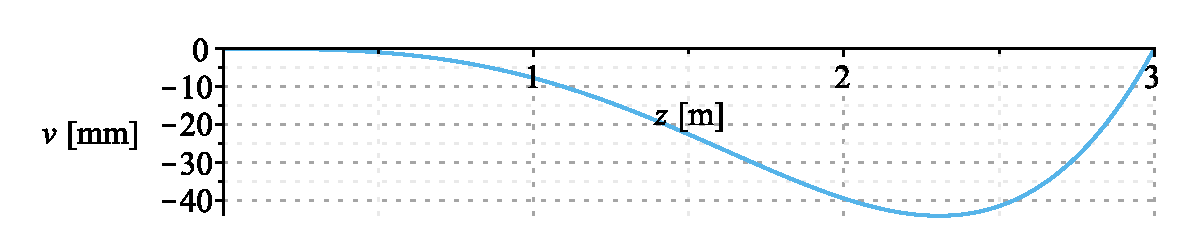
\includegraphics[width=0.7\linewidth]{displacement}
		\caption{vertical displacement of the turret from the nominal configuration.} \label{fig:displacement}
	\end{figure}

	The reported graph contradicts a requirement of our customer as the maximum displacements is bigger than $4cm$, exceeding the minimum target displacement value of $1cm$. This suggest that the chosen profile \texttt{10-040} is not able to withstand all the requirements. In order to avoid this problem two ways can be followed:
	\begin{itemize}
		\item use the mathematical model of the machine in the control system to compensate for such displacement;
		\item use a different profile with better response at deflection. Looking at the IPS catalogue, a suitable alternative is the \texttt{10-080} profile whose section is reported in figure \ref{fig:10-080}. Such beam is characterized by a moment of inertia $I_{xx} = 71.56cm^4$: neglecting the difference in weight contribution of the bar (whose density is increased to $\rho = 3.18kg/m$),  the maximum displacement is reduced to less then $6mm$, fully satisfying the customers requirement.
	\end{itemize}
	\begin{SCfigure}[3][bht]
		\centering
		\includegraphics[width=2.2cm]{10-080}
		\caption{section of the \texttt{10-080} T-slot profile by Parker IPS\cite{parker-ds}.}
		\label{fig:10-080}
	\end{SCfigure}
	
	In the following (and also in the final CAD) the solution based on the \texttt{10-040} profile is reported, however, due to the high \textit{modularity} provided by the T-slot profiles, assembling the machine with the \texttt{10-080} component will be practically the same.
	
	